\documentclass[sigconf,nonacm]{acmart}
\settopmatter{printacmref=false}
\pagestyle{plain}
\usepackage{booktabs}
\usepackage{balance}
\usepackage{pgfplots}
\usetikzlibrary{positioning,arrows.meta}
\pgfplotsset{compat=1.16}
% GENERATED by paper/make_numbers.py from measurements/data/rewrites.json -- do not edit by hand
\newcommand{\RWtotal}{130}
\newcommand{\RWsettled}{130}
\newcommand{\RWunsettled}{0}
\newcommand{\RWeq}{55}
\newcommand{\RWeqProven}{55}
\newcommand{\RWeqRefuted}{0}
\newcommand{\RWsimp}{75}
\newcommand{\RWbroken}{50}
\newcommand{\RWbrokenPct}{67}
\newcommand{\RWsimpEquiv}{25}
\newcommand{\RWbrokenSynth}{50}
\newcommand{\RWfaster}{20}
\newcommand{\RWfasterPct}{40}
\newcommand{\RWsmaller}{17}
\newcommand{\RWsmallerPct}{34}
\newcommand{\RWeither}{31}
\newcommand{\RWeitherPct}{62}
\newcommand{\RWloc}{46}
\newcommand{\RWlocDen}{46}
\newcommand{\RWlocPct}{100}
\newcommand{\RWgateMedian}{10.6}
\newcommand{\RWgateMax}{983.6}
\newcommand{\RWbaseArea}{82{,}326}
\newcommand{\RWbaseDelay}{24.50}
\newcommand{\RWbaseCells}{9{,}521}
\newcommand{\RWparts}{9{,}257}
\newcommand{\RWbmcChecked}{50}
\newcommand{\RWbmcConfirmed}{49}
\newcommand{\RWbmcTail}{: \textbf{every one} that is not a false rejection.}
\newcommand{\RWconfSynth}{49}
\newcommand{\RWconfEither}{30}
\newcommand{\RWconfEitherPct}{61}
\newcommand{\RWctlAny}{48}
\newcommand{\RWctlChecked}{48}
\newcommand{\RWctlConfirmed}{0}
\newcommand{\RWctlProven}{48}
\newcommand{\RWctlTimeout}{0}
\newcommand{\RWctlDead}{7}
\newcommand{\RWeqLive}{48}
\newcommand{\RWctlTop}{0}
\newcommand{\RWfalseRej}{1}
\newcommand{\RWsimpDead}{7}
\newcommand{\RWexOp}{fold guard}
\newcommand{\RWexFile}{ibex\_decoder.sv}
\newcommand{\RWexLine}{647}
\newcommand{\RWexOrig}{if (illegal\_c\_insn\_i)}
\newcommand{\RWexNew}{if (1'b1)}
\newcommand{\RWexGain}{19.0}
\newcommand{\RWexDelay}{19.85}
\newcommand{\AGanyState}{16}
\newcommand{\AGresetOnly}{1}
\newcommand{\AGproIters}{45}
\newcommand{\AGproLostPct}{33}
\newcommand{\AGworstLost}{9}
\newcommand{\AGworstIters}{15}
\newcommand{\AGworstPct}{60}
\newcommand{\AGbugs}{4}
\newcommand{\AGfalseRej}{17}
\newcommand{\AGfalseRejPct}{81}
\newcommand{\AGproGated}{42}
\newcommand{\AGproRef}{15}
\newcommand{\AGproFalse}{15}
\newcommand{\AGproBugs}{0}
\newcommand{\AGflashGated}{27}
\newcommand{\AGflashBugs}{4}
\newcommand{\AGflashFalse}{2}
\newcommand{\AGruns}{5}
\newcommand{\AGmodels}{2}
\newcommand{\AGiters}{85}
\newcommand{\AGgated}{69}
\newcommand{\AGrefused}{21}
\newcommand{\AGrefusedPct}{30}
\newcommand{\AGconfirmed}{4}
\newcommand{\AGrefFaster}{0}
\newcommand{\AGaccepted}{6}
\newcommand{\AGimproved}{5}
\newcommand{\AGbestPct}{11.2}
\newcommand{\AGbestFrom}{18.82}
\newcommand{\AGbestTo}{16.72}
\newcommand{\AGgateWarm}{13.9}
\newcommand{\AGgateCold}{86}
\newcommand{\AGcost}{13.01}
\newcommand{\AGiterMedian}{126}
\newcommand{\AGgateShare}{13}
\newcommand{\AGparts}{11{,}117}
\newcommand{\HProZero}{18.2}
\newcommand{\HProThirty}{22.6}
\newcommand{\HProOneTwenty}{28.0}
\newcommand{\HProSixHundred}{0.0}
\newcommand{\HProCells}{10}
\newcommand{\HFlashZero}{17.2}
\newcommand{\HFlashThirty}{8.0}
\newcommand{\HFlashOneTwenty}{0.7}
\newcommand{\HFlashSixHundred}{0.0}
\newcommand{\HFlashCells}{12}
\newcommand{\HProTurn}{162}
\newcommand{\HFlashTurn}{33}
\newcommand{\HProLoX}{0.7}
\newcommand{\HProHiX}{3.7}
\newcommand{\HFlashLoX}{0.9}
\newcommand{\HIsoZero}{11.1}
\newcommand{\HIsoThirty}{1.0}
\newcommand{\HIsoOneTwenty}{26.4}
\newcommand{\HIsoSixHundred}{18.5}
\newcommand{\HTwoVerdict}{not rejected}
\newcommand{\HTwoP}{0.11}
\newcommand{\HIsoSeeds}{3}
\newcommand{\HFiveLo}{1.4}
\newcommand{\HFiveHi}{2.6}
\newcommand{\HFiveDecided}{179}
\newcommand{\SSmedian}{6.3}
\newcommand{\SSpNinety}{13.1}
\newcommand{\PKGbestPct}{6.2}
\newcommand{\PKGbestNs}{16.93}
\newcommand{\PKGbestParent}{18.04}
\newcommand{\PKGbestS}{3}
\newcommand{\PKGrunPct}{4.1}
\newcommand{\PKGrunWould}{10.1}
\newcommand{\PKGfast}{3}
\newcommand{\PKGn}{12}
\newcommand{\PKGproven}{12}
\newcommand{\PKGtop}{10}
\newcommand{\PKGtopProven}{10}
\newcommand{\PKGtopS}{3}
\newcommand{\PKGtopMax}{17}
\newcommand{\PKGruns}{1}
\newcommand{\PKGrunsText}{all in one run}
\newcommand{\PKGenums}{\texttt{ctrl\_fsm\_e}, \texttt{exc\_pc\_sel\_e}, \texttt{imm\_b\_sel\_e}, \texttt{pc\_sel\_e}}
\newcommand{\ABctlRuns}{9}
\newcommand{\ABctlIters}{135}
\newcommand{\ABctlFalse}{35}
\newcommand{\ABctlRefused}{35}
\newcommand{\ABctlLostPct}{26}
\newcommand{\ABtrtRuns}{9}
\newcommand{\ABtold}{20}
\newcommand{\ABtoldReproven}{20}
\newcommand{\ABtoldFast}{0}
\newcommand{\ABruns}{46}
\newcommand{\ABmodels}{4}
\newcommand{\ABctlMed}{6.2}
\newcommand{\ABtrtMed}{6.5}
\newcommand{\ABscRuns}{18}
\newcommand{\ABscMed}{6.2}
\newcommand{\ABscTold}{81}
\newcommand{\ABscRefused}{82}
\newcommand{\ABscBugs}{1}
\newcommand{\ABgenSentence}{}
\newcommand{\ABscRest}{ (the other was a real bug, and it was refuted)}
\newcommand{\ABscSentence}{ With the final version of the sequential check (from reset, with package edits checked at the scope their changed types reach) in 18 more runs, 81 of 82 rejected edits came back proven and the agent was told so; the other was a real bug, refuted with a counterexample from reset. It proposed no package edit, and the median is 6.2\%.}
\newcommand{\ABacc}{69}
\newcommand{\ABaccReproven}{69}
\newcommand{\ABproBugs}{2}
\newcommand{\ABproGated}{488}
\newcommand{\TESTS}{448}


\begin{document}

\title{LiveLane: Formal Equivalence Checking Inside an Agentic RTL Loop
on a Whole RISC-V Core}

\author{Jayaraj Jayakumar}
\affiliation{\institution{UC Santa Cruz}\city{Santa Cruz}\state{CA}\country{USA}}
\email{jj8@ucsc.edu}

\begin{abstract}
An agent optimising RTL needs a formal equivalence check, and the standard
partition-based checker is least reliable on the strongest agent. LiveLane runs
an equivalence check and a sequential check, as composable CHIA nodes, on every
iteration of production
Gemini agents optimising a whole \texttt{ibex\_core}. Of \RWtotal{}
optimisation-style rewrites, \RWbmcConfirmed{} change what the edited module computes, and synthesis scores
\textbf{\RWconfEitherPct\%} of those as better than the original: an objective
that rewards removed logic also rewards incorrect logic. Across \ABctlRuns{}
runs of the strongest model, \textbf{all \ABctlFalse{} of the \ABctlRefused{}
edits the checker rejected were correct}, costing \ABctlLostPct\% of its
iterations. An unbounded sequential equivalence check (PDR) of the edited
instance from reset, at the parameters the core uses, proves them: in the loop,
\textbf{\ABscTold{} of \ABscRefused{} rejected edits were proven
correct}\ABscRest{}, and all \ABacc{} edits the loop accepted are re-proven
from any power-up state. With each package edit checked where its changed
types reach, the agent's re-encodings of shared enums are proven
\textbf{at the scope of the whole core}, among them the best edit of its
run, \textbf{\PKGbestPct\% faster and correct, which the checker rejected}. An
agent's tolerance to evaluator latency depends on the model: a slow reasoning
model tolerates delay up to a sharp threshold between 120\,s and 600\,s, a fast
one degrades steadily from under 30\,s, and latency costs the agent iterations,
not per-iteration quality. The check takes \AGgateWarm\,s per iteration, the
agent improves the core's critical path by up to \textbf{\AGbestPct\%} with
every accepted edit proven, and two partitioner fixes let eqy complete CVA6's
whole core: 280{,}764 partitions.
\end{abstract}

\keywords{agentic EDA, formal equivalence checking, RTL optimisation, CHIA}

\maketitle

\section{Introduction}

An agentic RTL loop proposes a rewrite, evaluates it, and keeps it if the
evaluation says it is better. The evaluation is usually simulation and synthesis
quality of results (QoR). Both are fast, and both err in the same direction: an
edit that removes logic tends to synthesise smaller and faster, whether or not
the removed logic mattered, so the objective rewards the incorrect rewrite.
Only formal equivalence checking rejects it, and the
RTL-editing loops of CHIA~\cite{chia} do not run one.

LiveLane adds one on every iteration of a production agent optimising a whole
RISC-V core, built as CHIA nodes that any RTL-editing loop can adopt. Our
results:

\begin{itemize}\setlength{\itemsep}{1pt}\setlength{\parskip}{0pt}
\item \textbf{Synthesis scores reward incorrect edits.} Synthesis scores
\RWconfEitherPct\% of the non-equivalent \texttt{ibex\_core} rewrites as better
than the original (\S\ref{sec:need}).
\item \textbf{The standard checker rejects correct edits.} Of the
\ABctlRefused{} \texttt{gemini-3.1-pro} edits it rejected, all \ABctlFalse{}
were correct (\S\ref{sec:right}).
\item \textbf{A sequential check resolves them in the loop.} An unbounded proof
from reset proved \ABscTold{} of \ABscRefused{} rejected edits inside the
loop\ABscRest{}, and re-proves all \ABacc{} accepted edits from any power-up
state (\S\ref{sec:closed}).
\item \textbf{Proofs beyond instance scope.} Enum re-encodings in the core's
shared package are proven at the scope of the whole core in seconds, including
a \PKGbestPct\%-faster edit the checker rejected (\S\ref{sec:right}).
\item \textbf{Latency requirement.} The check must be faster than the agent's
own turn, not a human's two seconds: latency costs an agent iterations, not
per-iteration quality (\S\ref{sec:fast}).
\item \textbf{Scale.} Two partitioner fixes take CVA6's whole core from zero
partitions to 280{,}764 (\S\ref{sec:cost}).
\end{itemize}
For CHIA, this moves formal verification from sign-off into the loop's critical
path: \texttt{LecGateNode} and \texttt{second\_stage} check any RTL edit with
open-source tools, and \texttt{DelayNode} lets any loop measure the cost of its
own evaluator latency.

\section{The loop and the equivalence check}
\label{sec:method}

\begin{figure}[t]
\centering
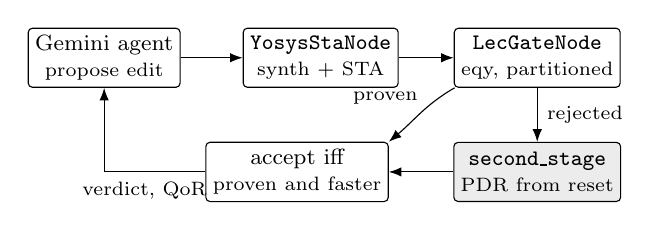
\begin{tikzpicture}[font=\footnotesize,
  box/.style={draw, rounded corners=1.5pt, align=center, inner sep=2.5pt,
              minimum height=7.5mm, minimum width=19mm},
  arr/.style={-{Latex[length=1.6mm]}}, lab/.style={font=\scriptsize}]
\node[box] (ag) at (0,0) {Gemini agent\\\scriptsize propose edit};
\node[box] (sy) at (2.75,0) {\texttt{YosysStaNode}\\\scriptsize synth + STA};
\node[box] (lec) at (5.5,0) {\texttt{LecGateNode}\\\scriptsize eqy, partitioned};
\node[box, fill=gray!15] (s2) at (5.5,-1.45) {\texttt{second\_stage}\\\scriptsize PDR from reset};
\node[box] (dec) at (2.45,-1.45) {accept iff\\\scriptsize proven and faster};
\draw[arr] (ag) -- (sy);
\draw[arr] (sy) -- (lec);
\draw[arr] (lec) -- node[lab, right] {rejected} (s2);
\draw[arr] (s2) -- (dec);
\draw[arr] (lec.200) to[out=210, in=40] node[lab, above left=-2pt, pos=0.45] {proven} (dec.north east);
\draw[arr] (dec.west) -| node[lab, below, pos=0.3] {verdict, QoR} (ag.south);
\end{tikzpicture}
\caption{The loop as a CHIA graph. Each box is a node declaring its own
resources; the scheduler places them. An edit is accepted only if proven.}
\label{fig:loop}
\end{figure}

One optimisation agent edits RTL. The equivalence check proves or refutes each
edit against its parent; a synthesis step scores it against one pinned sky130
Liberty library. An edit is kept only if it is proven equivalent and scores
better. The check is built on \texttt{eqy}, which splits two designs into
partitions and discharges each as an independent SMT obligation; every
partition's miter is flattened before solving, so no proof assumes another
partition equivalent. Around it we add an elaboration resolver, a
partition-level proof cache keyed on canonicalised RTLIL and on the query
settings (strategy, tool versions), and \texttt{DelayNode}, which adds a
controlled latency to any CHIA evaluator. The verdict is four-valued; only
\texttt{proven} accepts an edit, so a timeout is never treated as equivalence.

\section{Synthesis scores reward incorrect edits}
\label{sec:need}

\textbf{Instructions are not verification.} We ran \AGruns{} independent
optimisation runs of \AGmodels{} production models on the whole
\texttt{ibex\_core} (\AGiters{} iterations). The system prompt states that every
edit is checked for equivalence and that an edit changing behaviour is rejected:
\emph{``optimise the structure, not the function.''} Even so,
\texttt{gemini-2.5-flash} proposed \textbf{\AGflashBugs{} edits that change what
their module computes} among \AGflashGated{} that reached the check, each
refuted by a counterexample from reset (\S\ref{sec:right}) and each described by
the model as a restructuring (``refactored'', ``inlined''). \texttt{gemini-3.1-pro}
proposed none among \AGproGated{} here (\ABproBugs{} among \ABproGated{} in the
runs of \S\ref{sec:closed}). The error rate depends on the model; only a
formal check identifies the errors.

Rejected edits can also score better. \texttt{gemini-3.1-pro} proposed,
on \texttt{picorv32}, to ``factor [a] late signal to the top of the
logic tree''; simulation passed (1.31\,s), synthesis scored it
\textbf{13.8\% faster} (10.31 vs 11.97\,ns), and the check rejected it in
1.48\,s on \texttt{picorv32.mem\_done}. To measure how often a non-equivalent
edit is rewarded, we generate optimisation-style rewrites of a whole
\texttt{ibex\_core} (\RWbaseCells{} cells, \RWbaseArea\,\textmu m$^2$,
\RWbaseDelay\,ns critical path, \RWparts{} partitions, commit \texttt{23806e2};
the agent runs use the later pinned release, \AGbestFrom\,ns and \AGparts{}
partitions) in two families. \textbf{Equivalence-preserving} rewrites commute
the operands of \texttt{\&\&}, \texttt{||}, \texttt{\&} or \texttt{==}; the
checker must prove every one. \textbf{Simplifying} rewrites do what a
QoR-seeking agent does: drop a conjunct or disjunct, remove an inversion, fold
a guard to true, swap the two inputs of a multiplexer. Sites are sampled with a
fixed seed; every operator matches only a parenthesised expression of two simple
operands or a whole ternary right-hand side, so operand boundaries are
unambiguous. Sites in comments, in preprocessor branches excluded under the
defines in use, in loop bounds, on parameters, and on reset or clock nets are
excluded: these are structural edits no optimiser makes, and a rewrite that
holds every flip-flop in reset would collapse the core and trivially win on area.

\begin{center}\small
\begin{tabular}{@{}lr@{}}
\toprule
simplifying rewrites & \RWsimp \\
\quad rejected by the check & \textbf{\RWbroken} \\
\quad proven equivalent (edited logic dead or masked) & \RWsimpEquiv \\
rejected rewrites that synthesise & \RWbrokenSynth \\
\quad \textbf{scored better on QoR} (area or delay) & \textbf{\RWeither{} (\RWeitherPct\%)} \\
\quad faster critical path & \RWfaster{} (\RWfasterPct\%) \\
\quad smaller area & \RWsmaller{} (\RWsmallerPct\%) \\
\bottomrule
\end{tabular}
\end{center}

\begin{figure}[t]
\centering
\begin{tikzpicture}
\begin{axis}[
  width=\columnwidth, height=4.6cm,
  xlabel={\small $\Delta$ critical path vs original (\%)},
  ylabel={\small $\Delta$ area (\%)},
  xlabel near ticks, ylabel near ticks,
  tick label style={font=\footnotesize}, label style={font=\footnotesize},
  xmin=-21, xmax=14, ymin=-4.8, ymax=1.2,
  legend columns=2, legend style={font=\footnotesize, at={(0.5,1.03)}, anchor=south,
    draw=gray!50},
  grid=major, grid style={dotted,gray!40},
]
\fill[gray!12] (axis cs:-21,-4.8) rectangle (axis cs:0,0);
\node[font=\footnotesize,anchor=north west,gray!70!black]
  at (axis cs:-20.5,-3.9) {better on both};
\draw[gray!60] (axis cs:0,-4.8) -- (axis cs:0,1.2);
\draw[gray!60] (axis cs:-21,0) -- (axis cs:14,0);
\addplot[only marks, mark=x, mark size=2.6pt, thick, black]
  table[x=ddelay,y=darea] {scatter-refused.dat};
\addlegendentry{rejected by the check}
\addplot[only marks, mark=o, mark size=1.8pt, gray]
  table[x=ddelay,y=darea] {scatter-proven.dat};
\addlegendentry{proven equivalent}
\end{axis}
\end{tikzpicture}
\caption{Each simplifying rewrite of \texttt{ibex\_core} against the
original. A QoR-driven loop would keep the rejected rewrites left of or below
the axes, including the one with the largest timing gain.}
\label{fig:scatter}
\end{figure}

\textbf{\RWeitherPct\% of the rewrites the check rejects score better than the
original} (Fig.~\ref{fig:scatter}). A loop that accepts on QoR keeps all of
them. The largest single timing gain comes from a rejected rewrite: \RWexOp{} in
\texttt{\RWexFile}:\RWexLine, \texttt{\RWexOrig} $\rightarrow$
\texttt{\RWexNew}, which cuts the critical path by \RWexGain\% to
\RWexDelay\,ns. Synthesis is correct here: removing logic does make the
circuit faster. The objective is the problem, and only a semantic check fixes
it.

\section{Latency tolerance of the agent}
\label{sec:fast}

\begin{figure}[t]
\centering
\begin{tikzpicture}
\begin{axis}[
  width=0.95\columnwidth, height=3.3cm,
  ybar, bar width=7pt,
  symbolic x coords={0,30,120,600}, xtick=data,
  legend columns=2, legend style={font=\scriptsize, at={(0.5,1.03)}, anchor=south, draw=gray!50},
  legend image code/.code={\draw[#1] (0cm,-0.08cm) rectangle (0.2cm,0.08cm);},
  ymin=0, ymax=33,
  ylabel={\small improvement (\%)},
  xlabel={\small injected evaluator delay $d$ (s)},
  ylabel near ticks, xlabel near ticks,
  tick label style={font=\footnotesize}, label style={font=\footnotesize},
  grid=major, grid style={dotted,gray!40},
]
\addplot[draw=black,fill=black!70] table[x=delay,y=pro] {latency.dat};
\addlegendentry{gemini-3.1-pro}
\addplot[draw=black,fill=gray!30] table[x=delay,y=flash] {latency.dat};
\addlegendentry{gemini-2.5-flash}
\end{axis}
\end{tikzpicture}
\caption{Tolerance depends on the model. Critical-path improvement, fixed
1800\,s budget per run (\texttt{picorv32}, 2--3 seeds per condition). Turn
time: \HProTurn\,s (pro), \HFlashTurn\,s (flash); LiveSim's human target: 2\,s.}
\label{fig:cliff}
\end{figure}

LiveSim~\cite{livesim} targets two seconds because that is responsive for a
human user; an agent does not lose focus while it waits. We treat evaluator
latency as a controlled variable: condition $I(d)$ is the
identical tool stack plus $d$ seconds of injected delay, and the agent cannot
observe its condition (byte-identical prompts, no delay or clock field in its
context, both enforced by tests).

For \texttt{gemini-3.1-pro}, delays of 0, 30 and 120\,s give similar
outcomes and 600\,s finds no improvement (Fig.~\ref{fig:cliff}). Given the same
8 iterations, however, the 600\,s condition reaches \HIsoSixHundred\%, with no
significant difference across the four delays ($p=\HTwoP$): latency costs an
agent iterations, not per-iteration quality. This threshold depends on the
model, not on the tool. \texttt{gemini-2.5-flash}, whose turn takes
\HFlashTurn\,s against \HProTurn\,s for pro, falls from \HFlashZero\% to
\HFlashThirty\% at 30\,s and to \HFlashOneTwenty\% at 120\,s. Pro tolerates
delays up to \HProLoX$\times$ its own turn and finds no improvement at
\HProHiX$\times$, a sharp threshold; flash degrades steadily from
\HFlashLoX$\times$ its turn. For both, the bound is the model's own turn time:
the check need not reach LiveSim's two seconds, but must stay below the
agent's turn (minutes for a slow reasoning model, tens of seconds for a fast
one).

\section{Where formal checking spends its time}
\label{sec:cost}

On a XiangShan \texttt{Alu} iteration the equivalence check takes 54--77\% of
the wall time and synthesis 1--2\% (on \texttt{picorv32}, 14\% and 2\%), so the
check is the evaluator worth optimising. Within the check, on a whole
\texttt{ibex\_core} (12 corpus instances, 5{,}261--15{,}247 partitions):

\begin{center}\small
\begin{tabular}{@{}lrr@{}}
\toprule
phase & cold cache & warm cache \\
\midrule
\texttt{eqy -m} (elaborate + partition) & 100\,s & \textbf{148\,s} \\
prove & 228\,s & 25\,s \\
other & 60\,s & 54\,s \\
\midrule
\textbf{wall, 12 instances} & \textbf{388\,s} & \textbf{227\,s} \\
\bottomrule
\end{tabular}
\end{center}

Proving is 11\% of the cached run; \texttt{eqy -m} is 65.5\%, and partitioning
is 92\% of that step. \textbf{Roughly 60\% of the check's own run time is one
single-threaded C++ pass.} A proof cache removes only solver work: given the
warm run's other phases, the bound is 388/(227$-$25)\,=\,1.93$\times$, and we
measure 388/227\,=\,1.71$\times$.

Profiling that pass found a debug \emph{Fragment-Partition-Matrix} whose nested
loop over partitions $\times$ fragments issues one \texttt{log()} per cell,
unconditionally. Making it conditional takes \texttt{merge\_partitions} from
3.65\,s to 0.019\,s (190$\times$) and the partition step from 5.36\,s to
1.72\,s (3.1$\times$). The same defect explained a result we had recorded as a
scaling limit: CVA6's whole core produced \textbf{zero} partitions in 17\,min
while writing a 2.2\,GB log. A second defect also blocked it: generate-block
nesting produced partition names longer than the 255-byte filename limit,
aborting after 214{,}903 partitions. With both fixed (names over 100 characters
become an FNV-1a digest plus a readable tail; 74{,}005 shortened,
\textbf{zero collisions}), the partitioner completes \texttt{picorv32} (590
partitions), \texttt{ibex\_core} (5{,}261--15{,}247), XiangShan
\texttt{DivUnit} (16{,}065) and \textbf{CVA6's whole core: 280{,}764 partitions
in 790\,s}. Both limits were defects in the tool, not properties of the design.

\section{Accuracy of the check}
\label{sec:right}

\textbf{The partition-based check rejects correct edits.} A partition-based
checker cuts the design at signals it matches between the two sides and proves
each partition with those cut points as free inputs, so a cut errs towards
rejection: an edit that redefines a matched internal net while preserving every
output is rejected on that net. Of the agent's \AGrefused{} rejected edits,
\textbf{\AGfalseRej{} (\AGfalseRejPct\%) are correct}, including
\textbf{all \AGproRef{} of \texttt{gemini-3.1-pro}'s}. Its rewrites of the
fetch FIFO substitute the definition of \texttt{out\_valid\_o} into
\texttt{pop\_fifo}; eqy cuts at \texttt{out\_valid\_o}, treats it as a free
input, and rejects \texttt{fifo\_i.pop\_fifo}, the only failing partition. All
\AGfalseRej{} are proven from reset for any power-up state, and \AGanyState{}
also without reset, from any shared initial state.

\textbf{A sequential check resolves them.} On a rejection, we check the edited
instance against its parent with an unbounded sequential engine (PDR), falling
back to bounded model checking for a counterexample when PDR times out. The
initial state is explicit: both copies start in the same arbitrary state
(register pairs matched by name and width) and reset is asserted in the first
cycle; a second proof omits the reset. The common shortcut, starting both copies from all-zero,
is both unsound and incomplete: it accepts an edit that relies on un-reset
flip-flops powering up to zero, and refutes a one-hot state machine, whose
all-zero state is illegal. The instance is extracted from the whole core
elaborated with hierarchy preserved, so it carries the parameters the core
gives it; checked standalone at default parameters, one agent edit to
\texttt{ibex\_counter} is reported proven although it breaks the core's
\texttt{minstret} counter. The sequential check resolves all
\AGrefused{}~+~\RWbroken{} rejections at a median of \SSmedian\,s each (90th
percentile \SSpNinety\,s): it refutes \AGbugs{} agent edits and
\RWbmcConfirmed{} rewrites with counterexamples from reset, and proves
\AGfalseRej{} agent edits and \RWfalseRej{} rewrite correct. A refutation holds
at instance scope: the module computes something different, but the core need
not exercise the difference; three LSU rewrites that drop
\texttt{|| pmp\_err\_q} are correct in this core, whose PMP is disabled.
It proves all \RWctlProven{} equivalence-preserving rewrites of instantiated
logic from any shared initial state, with \textbf{\RWctlConfirmed{}}
counterexamples. Restricted to confirmed bugs, synthesis still scores
\RWconfEither{} of \RWconfSynth{} (\textbf{\RWconfEitherPct\%}) better than the
original.

\textbf{Edits to a shared package.} Some of the stronger model's edits change no
module: \PKGn{} re-encode enums in \texttt{ibex\_pkg} (\PKGenums),
\PKGrunsText. A package has no instance to extract; eqy accepted none, nor could
the initial version of the sequential check (all-zero initial state, instance
scope). We check such an edit at the scope its changed types reach: one module
at its instances, or the top level for a type carried across ports. \textbf{\PKGproven{} of \PKGn{} are proven correct},
\PKGtopProven{} at the scope of the whole core (median \PKGtopS\,s, at most
\PKGtopMax\,s): with every register matched, we use register
correspondence~\cite{vaneijk}, replacing each register pair with one shared free
value and proving one cycle, so unchanged logic merges away; the same method
fails, as it must, on a moved CSR address. A one-hot controller state machine,
whose state register has no counterpart, is proven from reset by PDR.
\PKGfast{} were faster; the best scored \PKGbestNs\,ns against the
\PKGbestParent\,ns of its parent, \textbf{\PKGbestPct\%, the best edit of its
run}, which ended at \PKGrunPct\%; this edit alone would take it to
\PKGrunWould\%.

\textbf{Real bugs and localisation.} On 12 merged
\texttt{lowRISC/\allowbreak ibex} bug-fix pull requests, each checked at its own
base commit, the check refutes 11 of 12; the twelfth (\#1780) fixes PMP logic
this configuration never instantiates. Preserving module hierarchy through the
front end (\texttt{read\_slang --keep-hierarchy}) moves partition cuts onto
module ports:

\begin{center}\small
\begin{tabular}{@{}lrr@{}}
\toprule
 & flattened & hierarchical \\
\midrule
verdict agreement & \multicolumn{2}{c}{\textbf{12 / 12}} \\
failing partitions in the changed module & 47.2\% & \textbf{100\%} \\
distinct modules implicated (mean) & 2.18 & \textbf{1.00} \\
partitions & 9{,}110 & \textbf{6{,}022} \\
checked iteration, median & 20.6\,s & \textbf{15.2\,s} \\
\bottomrule
\end{tabular}
\end{center}

Flattened checking finds the same nets but reports them wherever the
partitioner cut (on one instance, in five modules the patch never touched).
Hierarchical checking attributes \textbf{every one of 55} failing partitions to
the module that produced the difference. On the rewrites, all \RWbroken{}
rejections fail only inside the rewritten module (\RWloc{} matched
automatically, the rest by partition name).

\section{The complete loop}
\label{sec:closed}

Across the runs of \S\ref{sec:need}, \AGimproved{} of \AGruns{} improved \texttt{ibex\_core}'s critical path, by up to \textbf{\AGbestPct\%}
(\AGbestFrom\,ns $\rightarrow$ \AGbestTo\,ns), through \AGaccepted{} accepted
edits, each proven equivalent to its parent before acceptance. The check
took \textbf{\AGgateWarm\,s} per iteration (warm cache) over \AGparts{}
partitions (\AGgateCold\,s at most on a cold first proof), about
\AGgateShare\% of a median \AGiterMedian\,s iteration and well below the
threshold of \S\ref{sec:fast}. Total model cost was \$\AGcost. We then ran the
sequential check in the loop: \ABtrtRuns{} runs of \texttt{gemini-3.1-pro} with
its initial version (all-zero initial state, instance scope), \ABctlRuns{}
without it. Without it, correct edits that eqy rejected took \ABctlLostPct\% of
the model's iterations. With it, the agent was told \ABtold{} times that a
rejected edit was correct (all \ABtoldReproven{} re-proven from reset), but
those rewrites were never faster, and the median improvement barely changes
(\ABtrtMed\% vs \ABctlMed\%): the check changed what the agent was told, not
what it kept. The faster correct edits were the enum re-encodings, provable
only at the scope of their types (\S\ref{sec:right}).\ABscSentence{}\ABgenSentence{}
Every edit the loop accepted in these runs is re-proven from reset: \ABaccReproven{} of \ABacc{}.

\section{Contribution to CHIA}

The track asks for agentic formal verification on a large RTL IP block.
LiveLane applies it to a whole RISC-V core on every iteration: \AGparts{}
partitions of \texttt{ibex\_core} proven per edit in \AGgateWarm\,s, inside a
CHIA graph whose nodes declare their own resources. Three components carry over
to any CHIA loop that edits RTL. \texttt{LecGateNode} accepts an edit only if
it is proven. \texttt{second\_stage} turns the checker's rejections into proofs
or counterexamples from reset, so the agent receives a correct verdict, which
matters most for the strongest models. \texttt{DelayNode} makes evaluator
latency an experimental variable, so a loop can measure the speed it needs. All of it runs on open-source tools
(Yosys, eqy, SymbiYosys, OpenSTA), with no commercial licence in the loop.

\section{Related work}

Scalable equivalence checking merges internal nets proven equal and treats them
as cut points~\cite{kuehlmann}; sequential checkers exploit the same structural
similarity~\cite{vaneijk}. The false rejections of \S\ref{sec:right} are the
known cost of that abstraction. We show where it occurs in agentic loops: an LLM
that substitutes a signal's definition into a logic cone produces exactly such
edits, and the stronger model produced more. Our sequential check is
unbounded model checking~\cite{bradley,een} per instance, at the design's own
parameters. The flow is built on Yosys~\cite{yosys}, eqy and SymbiYosys; the
cores are Ibex~\cite{ibex} and CVA6~\cite{cva6}. LiveSim~\cite{livesim} targets
two seconds for humans; \S\ref{sec:fast} measures an agent.

\section{Scope}

The equivalence-checking results are on \texttt{ibex} (\ABruns{} agent runs,
\ABmodels{} Gemini models, plus the rewrite campaign); the latency study is on
\texttt{picorv32}. Sequential proofs take free inputs at their scope's boundary,
so a proof covers every input the rest of the core could supply, and a
refutation shows only that the logic within that scope changed.

\section{Artifact and reproducibility}

The loop is five CHIA nodes, each declaring its own resources and usable
alone: \texttt{LecGateNode} and \texttt{second\_stage}
(\texttt{eqy}), \texttt{YosysStaNode}, \texttt{VerilatorSimNode} and
\texttt{DelayNode}. Any RTL-editing CHIA loop can adopt the two formal nodes
unchanged; \texttt{DelayNode} lets any loop measure how much evaluator latency
its agent tolerates. The artifact contains the loop, the nodes, the rewrite
generator, the re-checker for every rejection, the corpus harness, the
partitioner fixes as a patch, and every cited measurement file; a script
generates the paper's numbers for the rewrite campaign, agent runs, sequential
check and latency study from those files. \TESTS{} tests pass with the real
tools on \texttt{PATH}; CI runs the formal tests, including the whole-core proofs, on every push with the unmodified OSS
CAD Suite.

\section*{Acknowledgement of AI assistance}

Claude, Gemini was used for writing and refactoring code, running and analysing
the measurement campaign. All experimental design decisions, all measurements,
and the final content are by human.

\begin{thebibliography}{9}
\footnotesize
\bibitem{livesim} H. Skinner, R. T. Possignolo, S. Wang, and J. Renau.
LiveSim: A Fast Hot Reload Simulator for HDLs. \emph{ISPASS}, 2020.
\bibitem{chia} CHIA: an open framework for agentic HW/SW co-design flows.
\url{https://chialoops.ai}.
\bibitem{kuehlmann} A. Kuehlmann and F. Krohm. Equivalence checking using cuts
and heaps. \emph{DAC}, 1997.
\bibitem{vaneijk} C. A. J. van Eijk. Sequential equivalence checking based on
structural similarities. \emph{IEEE TCAD}, 19(7), 2000.
\bibitem{bradley} A. R. Bradley. SAT-based model checking without unrolling.
\emph{VMCAI}, 2011.
\bibitem{een} N. E\'en, A. Mishchenko, and R. Brayton. Efficient implementation
of property directed reachability. \emph{FMCAD}, 2011.
\bibitem{yosys} C. Wolf. Yosys Open SYnthesis Suite.
\url{https://yosyshq.net/yosys/}.
\bibitem{ibex} lowRISC. Ibex RISC-V core. \url{https://github.com/lowRISC/ibex}.
\bibitem{cva6} F. Zaruba and L. Benini. The cost of application-class
processing: energy and performance analysis of a Linux-ready 1.7-GHz 64-bit
RISC-V core in 22-nm FDSOI technology. \emph{IEEE TVLSI}, 27(11), 2019.
\end{thebibliography}

\balance
\end{document}
